Wie eben diskutiert, koppelt die starke Wechselwirkung an Teilchen, die Farbladung tragen.
Die Farbladung hat hierbei drei mögliche Zustände: rot, blau und grün.
Dabei spielt der Zustand der Farbladung für die Stärke der starken Wechselwirkung keine Rolle.
Zusätzlich zu den drei Zuständen der Farbladung gibt es auch drei Zustände der Antifarbladung: antirot, antiblau und antigrün.
\newline
Die Kombination der drei (Anti-)Farbladungen, oder die Kombination von Farbladung mit ent\-spre\-chender Antifarbladung, ergibt, angelehnt an die Farblehre, weiß.
Teilchen mit einer solchen Kombination der Farbladung ergeben entsprechend nach außen hin farbneutrale Teilchen, auch wenn sie aus farbgeladenen Teilchen aufgebaut sind.
\newline
Quarks, Antiquarks und Gluonen tragen Farbladung, wodurch sie an der starken Wechselwirkung teilnehmen.
Unter anderem bindet die starke Wechselwirkung Quarks und Antiquarks zu  Hadronen.
Diese werden wiederum in  Baryonen, aufgebaut aus drei Quarks, und  Mesonen, aufgebaut aus einem Quark-Antiquark-Paar, und entsprechende Antiteilchen, unterteilt.
\newline
Die Wechselwirkung zur Bindung eines Quark-Antiquark-Paars folgt dabei einem Potential $V(r)$ \cite{script:kt1}:
\begin{align} \label{eq:Potential}
V(r) = -\frac{4}{3}\frac{\alpha_\text{s}}{r} + kr 
\end{align}
Der erste Teil $-\frac{4}{3}\frac{\alpha_\text{s}}{r}$ verhält sich proportional zur  Kopplungskonstanten der starken Wechselwirkung $\alpha_{\text{s}}$ und antiproportional zum Abstand $r$ zwischen Quark und Antiquark.
\newline
Der zweite Teil des Potentials $+kr$ weist eine lineare Abhängigkeit von $r$ auf.
Der Vorfaktor $k$ wird als Stringspannung bezeichnet und liegt in der Größenordnung von etwa 1 GeV/fm \cite{Zheng:2018yxq}.
Für große Abstände dominiert der lineare Teil.
Das Feld der starken Wechselwirkung zwischen den beiden Teilchen wird immer stärker und wird deshalb als \textit{String} bezeichnet.
Für kleine $r$ nähert sich $V(r)$ einem Coulombpotential.
\newline
Um den Abstand zwischen sich zu vergrößern, müssen die zwei Teilchen immer mehr Energie besitzen, die insgesamt der Energie des \textit{String} entspricht.
Ab einem bestimmten Abstand reicht die Energie in dem \textit{String} aus, um ein weiteres Quark-Antiquark-Paar zu erzeugen.
In dem String bildet sich ein neues Quark-Antiquark-Paar, das sich mit dem ursprüngliche Quark-Antiquark-Paar zu zwei Quark-Antiquark-Paaren kombiniert.
Es liegen dann zwei Quark-Antiquark-Paare vor, die jeweils aus einem ursprünglichen Teilchen und einem neu entstandenen Teilchen bestehen.
Deshalb können Quarks nur in gebundenen Zuständen gemessen werden.
Dieses Phänomen wird als \textit{Con\-fine\-ment} bezeichnet.
Aus dem \textit{Confinement} folgt, dass in der Natur nur farbneutrale Teilchen frei vorkommen, sprich (Anti-)Quarks bilden immer andere Teilchen.%
\newline
Anders als die Bezeichnung vermuten lässt, ist $\alpha_\text{s}$ nicht konstant, sondern abhängig von der Auf\-lö\-sung, mit der die Wechselwirkung betrachtet wird.
Je genauer die Auflösung wird, umso kleiner wird $\alpha_{\rm{s}}$.
Aufgrund dieses Verhaltens von $\alpha_{\rm{s}}$ bezüglich der Auflösung nennt man $\alpha_\text{s}$ auch laufende Kopplungskonstante.
Farbgeladene Teilchen spüren für eine genaue Auflösung beziehungsweise kleines $\alpha_\text{s}$ nur eine kleine Wechselwirkung.
\newline
Halten sich viele (Anti-)Quarks und Gluonen auf kleinem Raum auf, so befindet sich ein Teilchen immer nah an einem anderen Teilchen.
Dadurch können sich die Teilchen innerhalb eines solchen Zustands quasi frei bewegen.
Den Zustand, wenn sich farbgeladene Teilchen frei bewegen können, nennt man asymptotische Freiheit.
Eine theoretische Beschreibung eines solchen Zustands ist das  Quark-Gluon-Plasma (QGP).
Das QGP entspricht einem Medium mit hoher Dichte von (Anti"~)""Quarks und Gluonen und be\-zie\-hungs\-wei\-se oder hoher Temperatur.
\newline
Ein solcher heißer und dichter Zustand kann kurz nach der Kollision von zwei hochenergetischen Atomkernen entstehen \cite{Karsch:2006xs}.
In der Überlappregion der beiden Atomkerne bildet sich ein QGP aus, das expandiert und abkühlt.
Durch das Expandieren und Abkühlen ändert sich der Zustand des Mediums und die farbgeladenen Teilchen schließen sich in der  Hadronisierung wieder zu Hadronen zusammen.
Bei dem beschriebene Übergang des QGP in hadronische Materie handelt es sich um einen Phasenübergang stark wechselwirkender Materie.
\begin{figure}[tp]
\centering
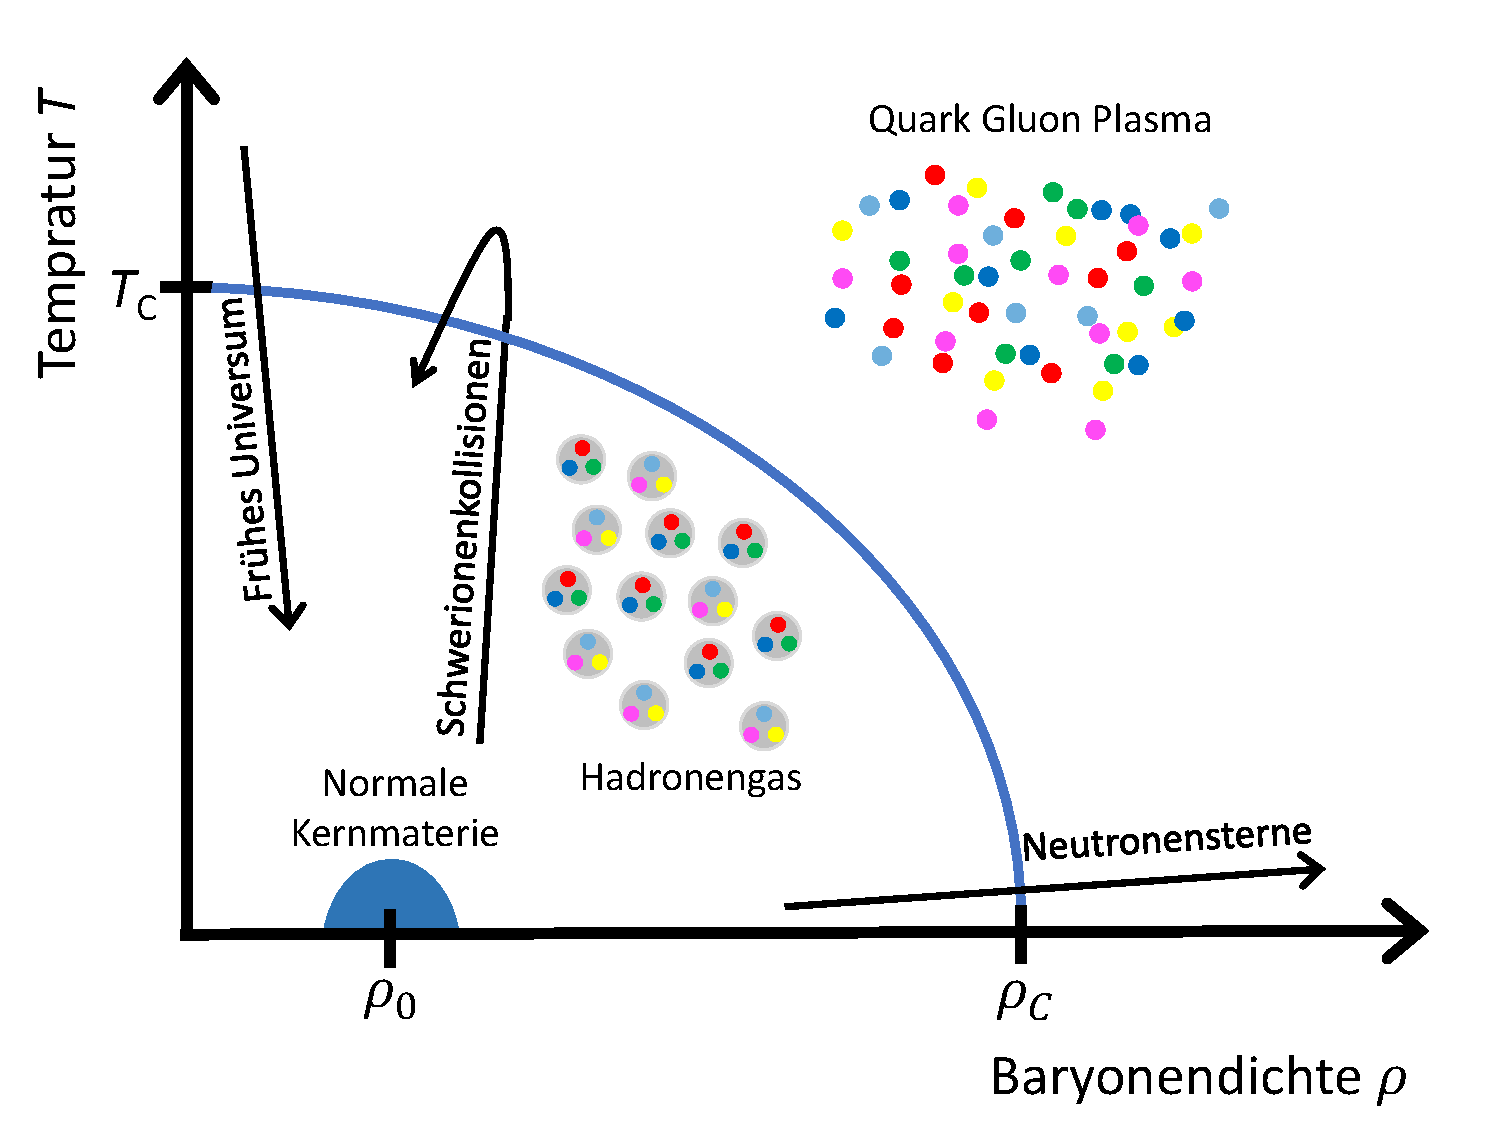
\includegraphics[width=.6\linewidth]{QCD_phase_diagram.pdf}
\caption{Phasendiagramm stark wechselwirkender Materie in Abhängigkeit der Baryonendichte $\rho$ und der Temperatur $T$.
\cite{Thesis:Tim}}
\label{fig:QGPPhase}
\end{figure}
\newline
Für die Erforschung des QGP spielt das Phasendiagramm stark wechselwirkender Materie eine wichtige Rolle.
Abbildung \ref{fig:QGPPhase} skizziert dieses in Abhängigkeit von der Baryonendichte $\mu_{\text{B}}$ und der Temperatur $T$.
Bei geringem $\mu_{\text{B}}$ und niedrigem $T$, wie etwa Raumtemperatur, sind alle Quarks und Gluonen in Hadronen gebunden.
Erhöht man $T$ oder beide Größen stark, wird ein Übergang in das QGP erwartet, in dem sich die Quarks und Gluonen quasi frei bewegen können.
Außerdem muss die Energiedichte groß genug sein, um ein QGP erzeugen zu können, weshalb davon ausgegangen wird, dass im frühen Universum kurz nach dem Urknall die gesamte Materie als QGP vorlag \cite{Kapusta:2000fe}. 
Es wird außerdem angenommen, dass sich dieses bei Kern-Kern-Kollisionen im Labor ausbilden kann, wie sie beim \textit{\textbf{A} \textbf{L}arge \textbf{H}adron \textbf{C}ollider \textbf{E}xperiment} (ALICE) untersucht werden.
\newline
Zum besseren Verständnis von Kern-Kern-Kollisionen werden auch Proton-Proton-Kollisionen (pp-Kollisionen) studiert.
Letztere werden in dieser Arbeit analysiert und im folgenden Abschnitt näher erläutert.